\section{Results}

\begin{figure}
\centering
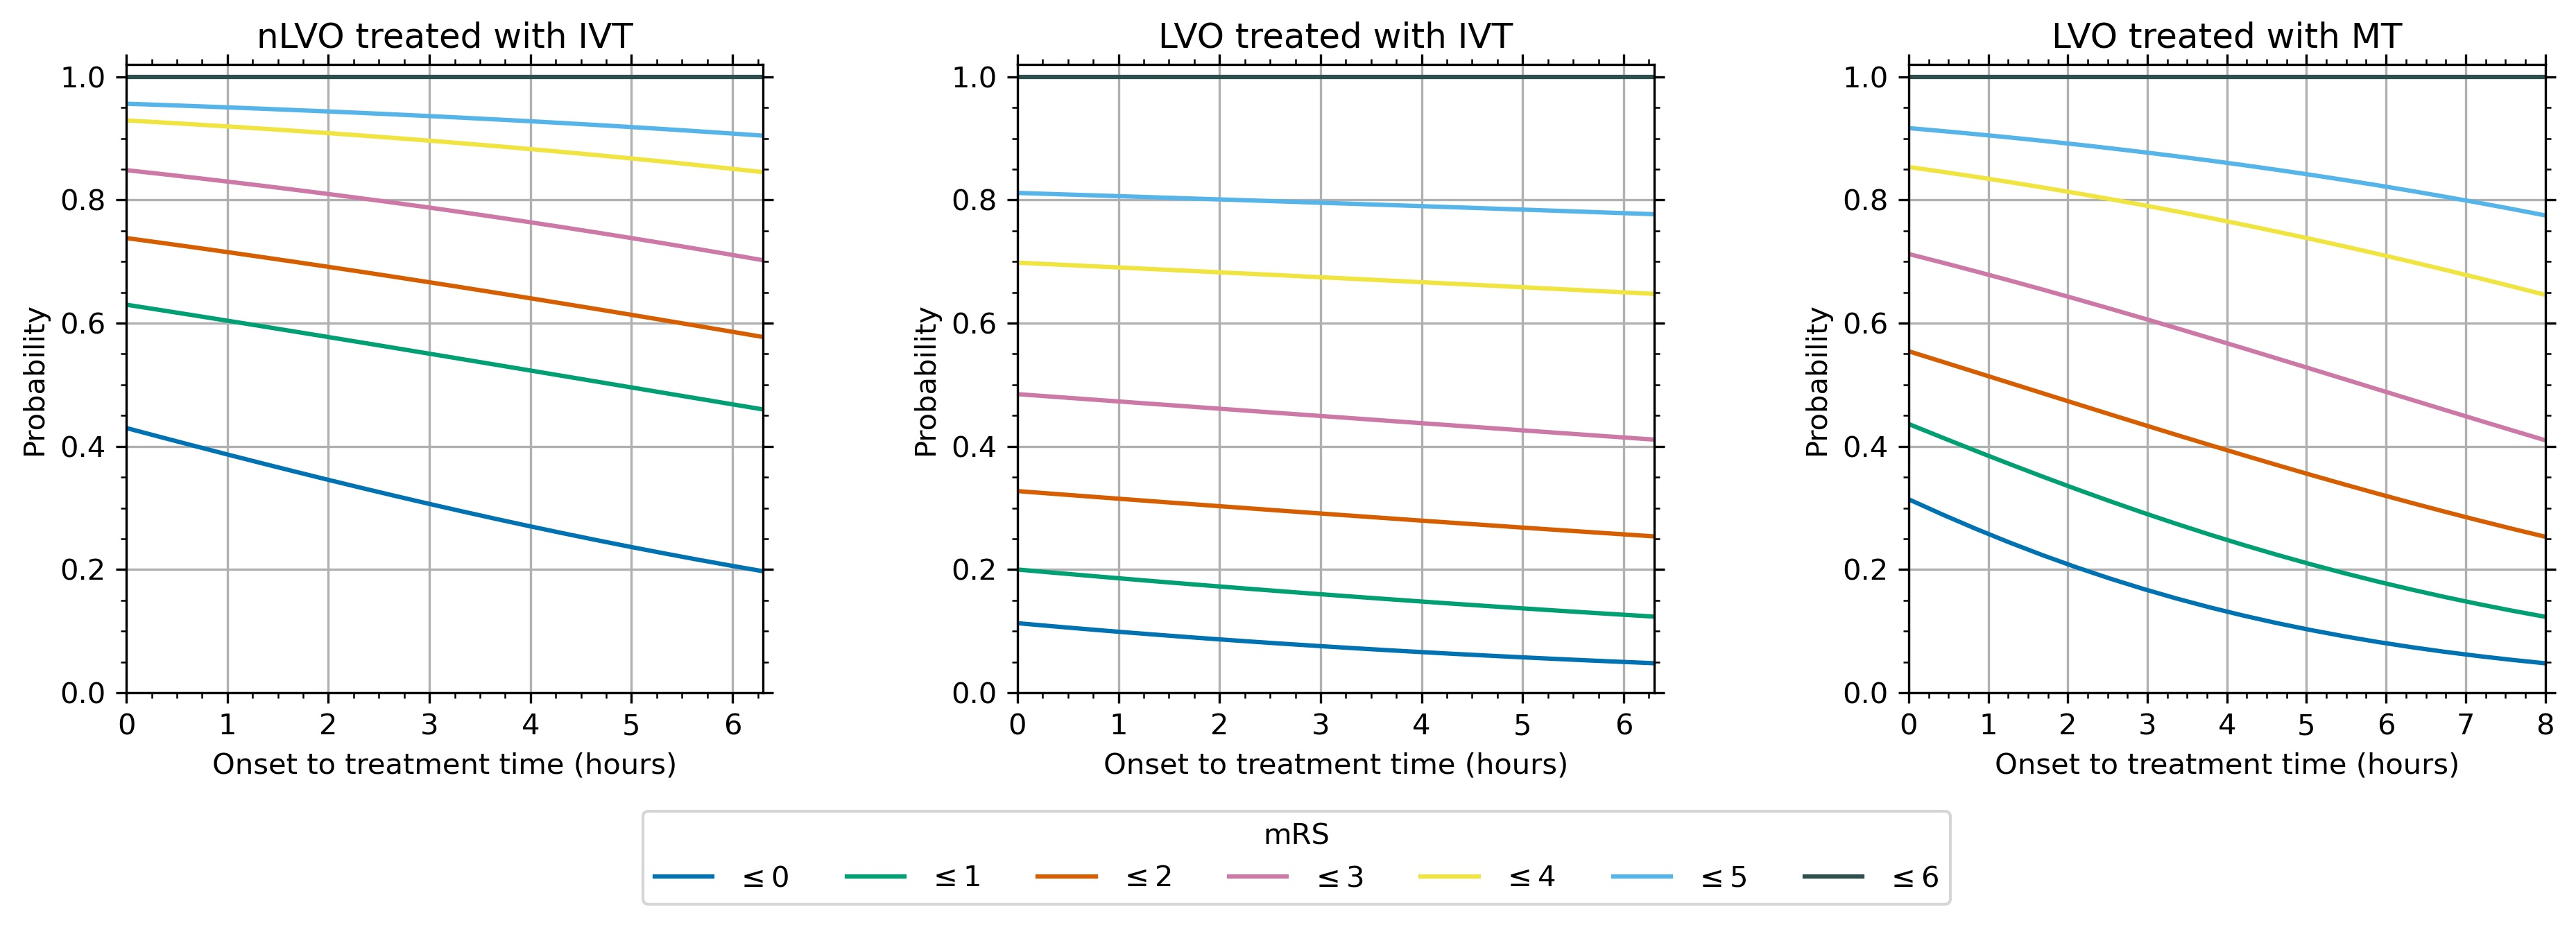
\includegraphics[width=\textwidth]{./images/probs_with_time}
\caption{mRS probability distributions by time from onset to treatment. Left: nLVO treated with IVT. Middle: LVO treated with IVT. Right: LVO treated with MT.}
\label{fig:probs_with_time_1}
\end{figure}

\begin{figure}
\centering
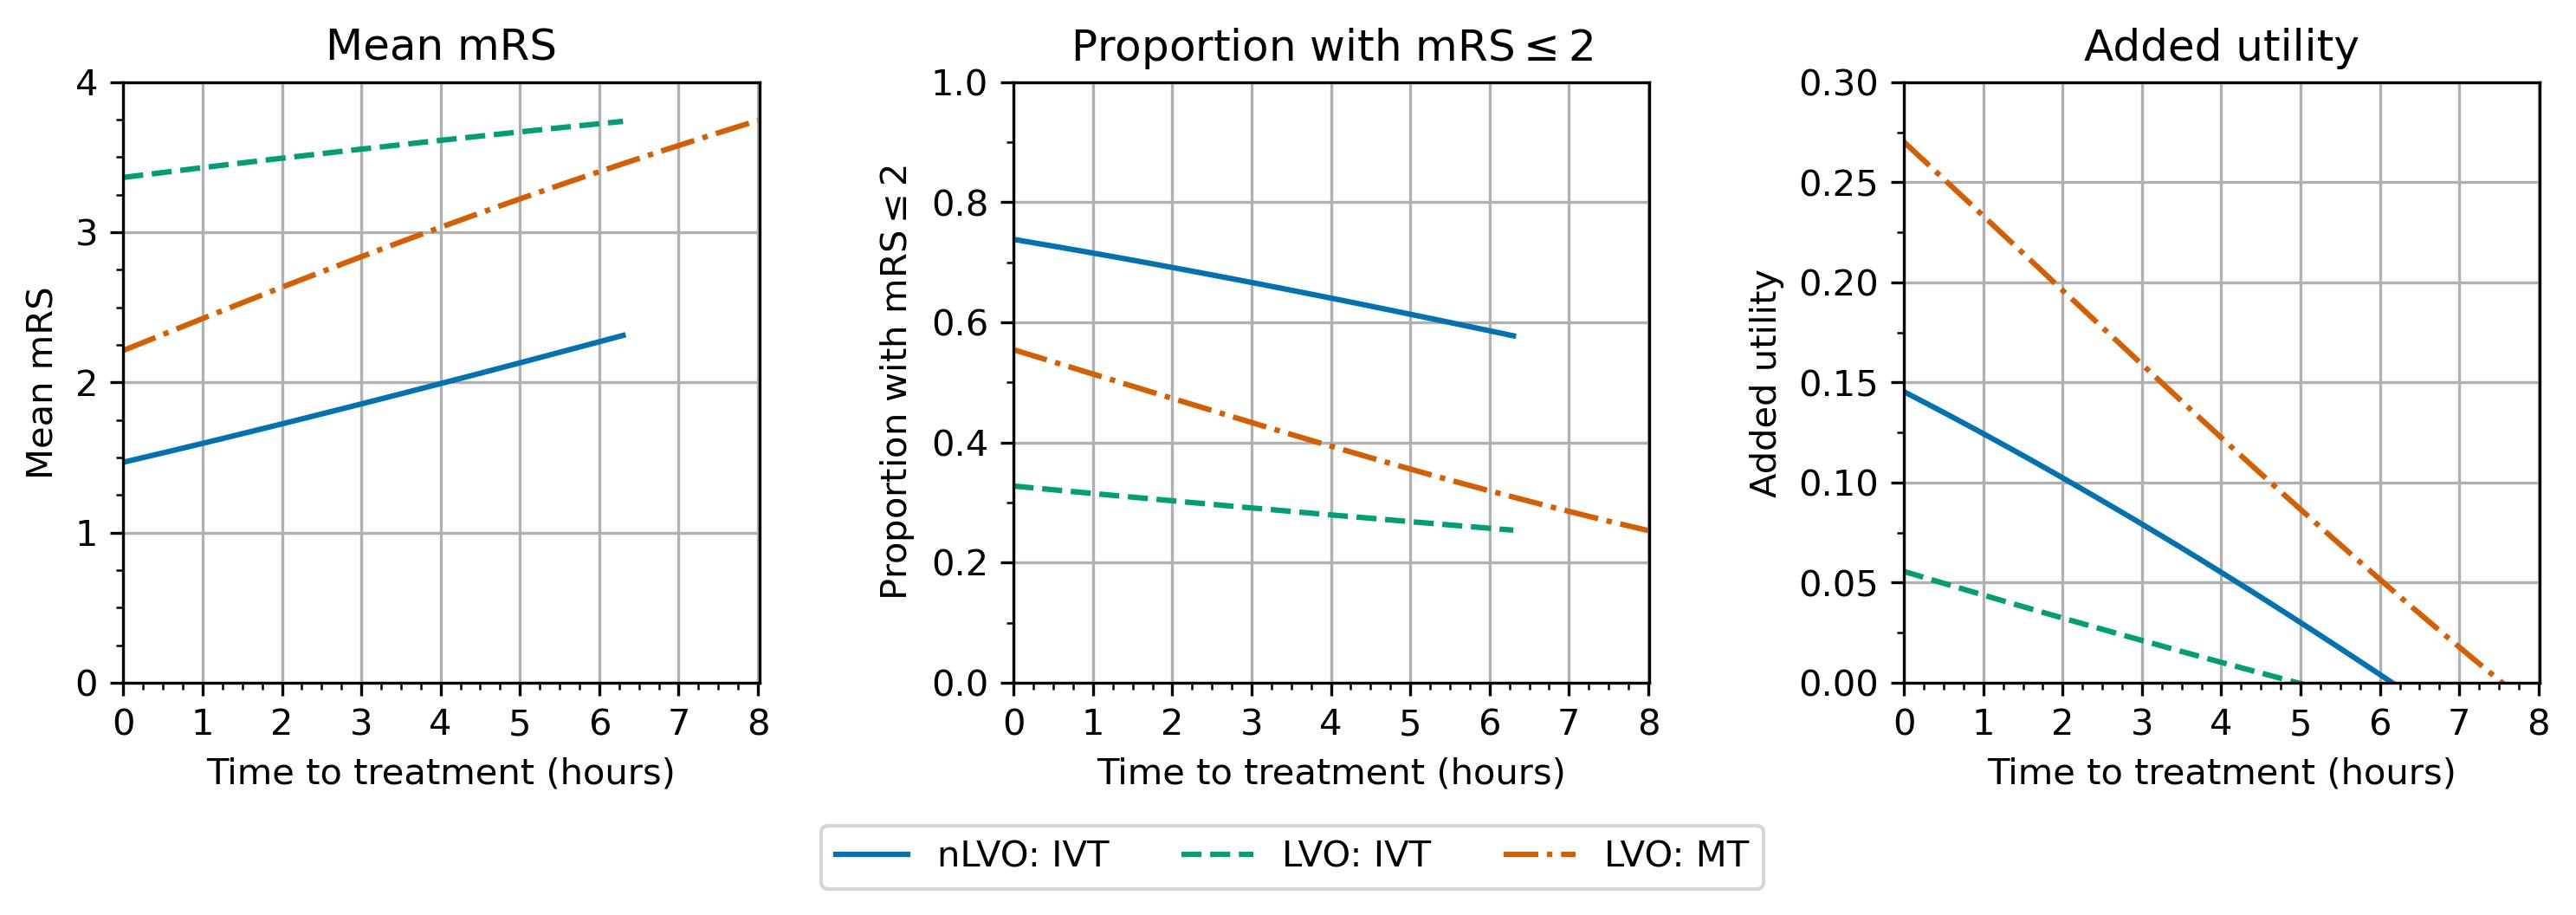
\includegraphics[width=\textwidth]{./images/time_to_treatment}
\caption{Alternative outcome measures by by time from onset to treatment. Left: mean mRS. Middle: Proportion of patients with mRS 0-2. Right: Added utility.}
\label{fig:probs_with_time_2}
\end{figure}

\begin{figure}
\centering
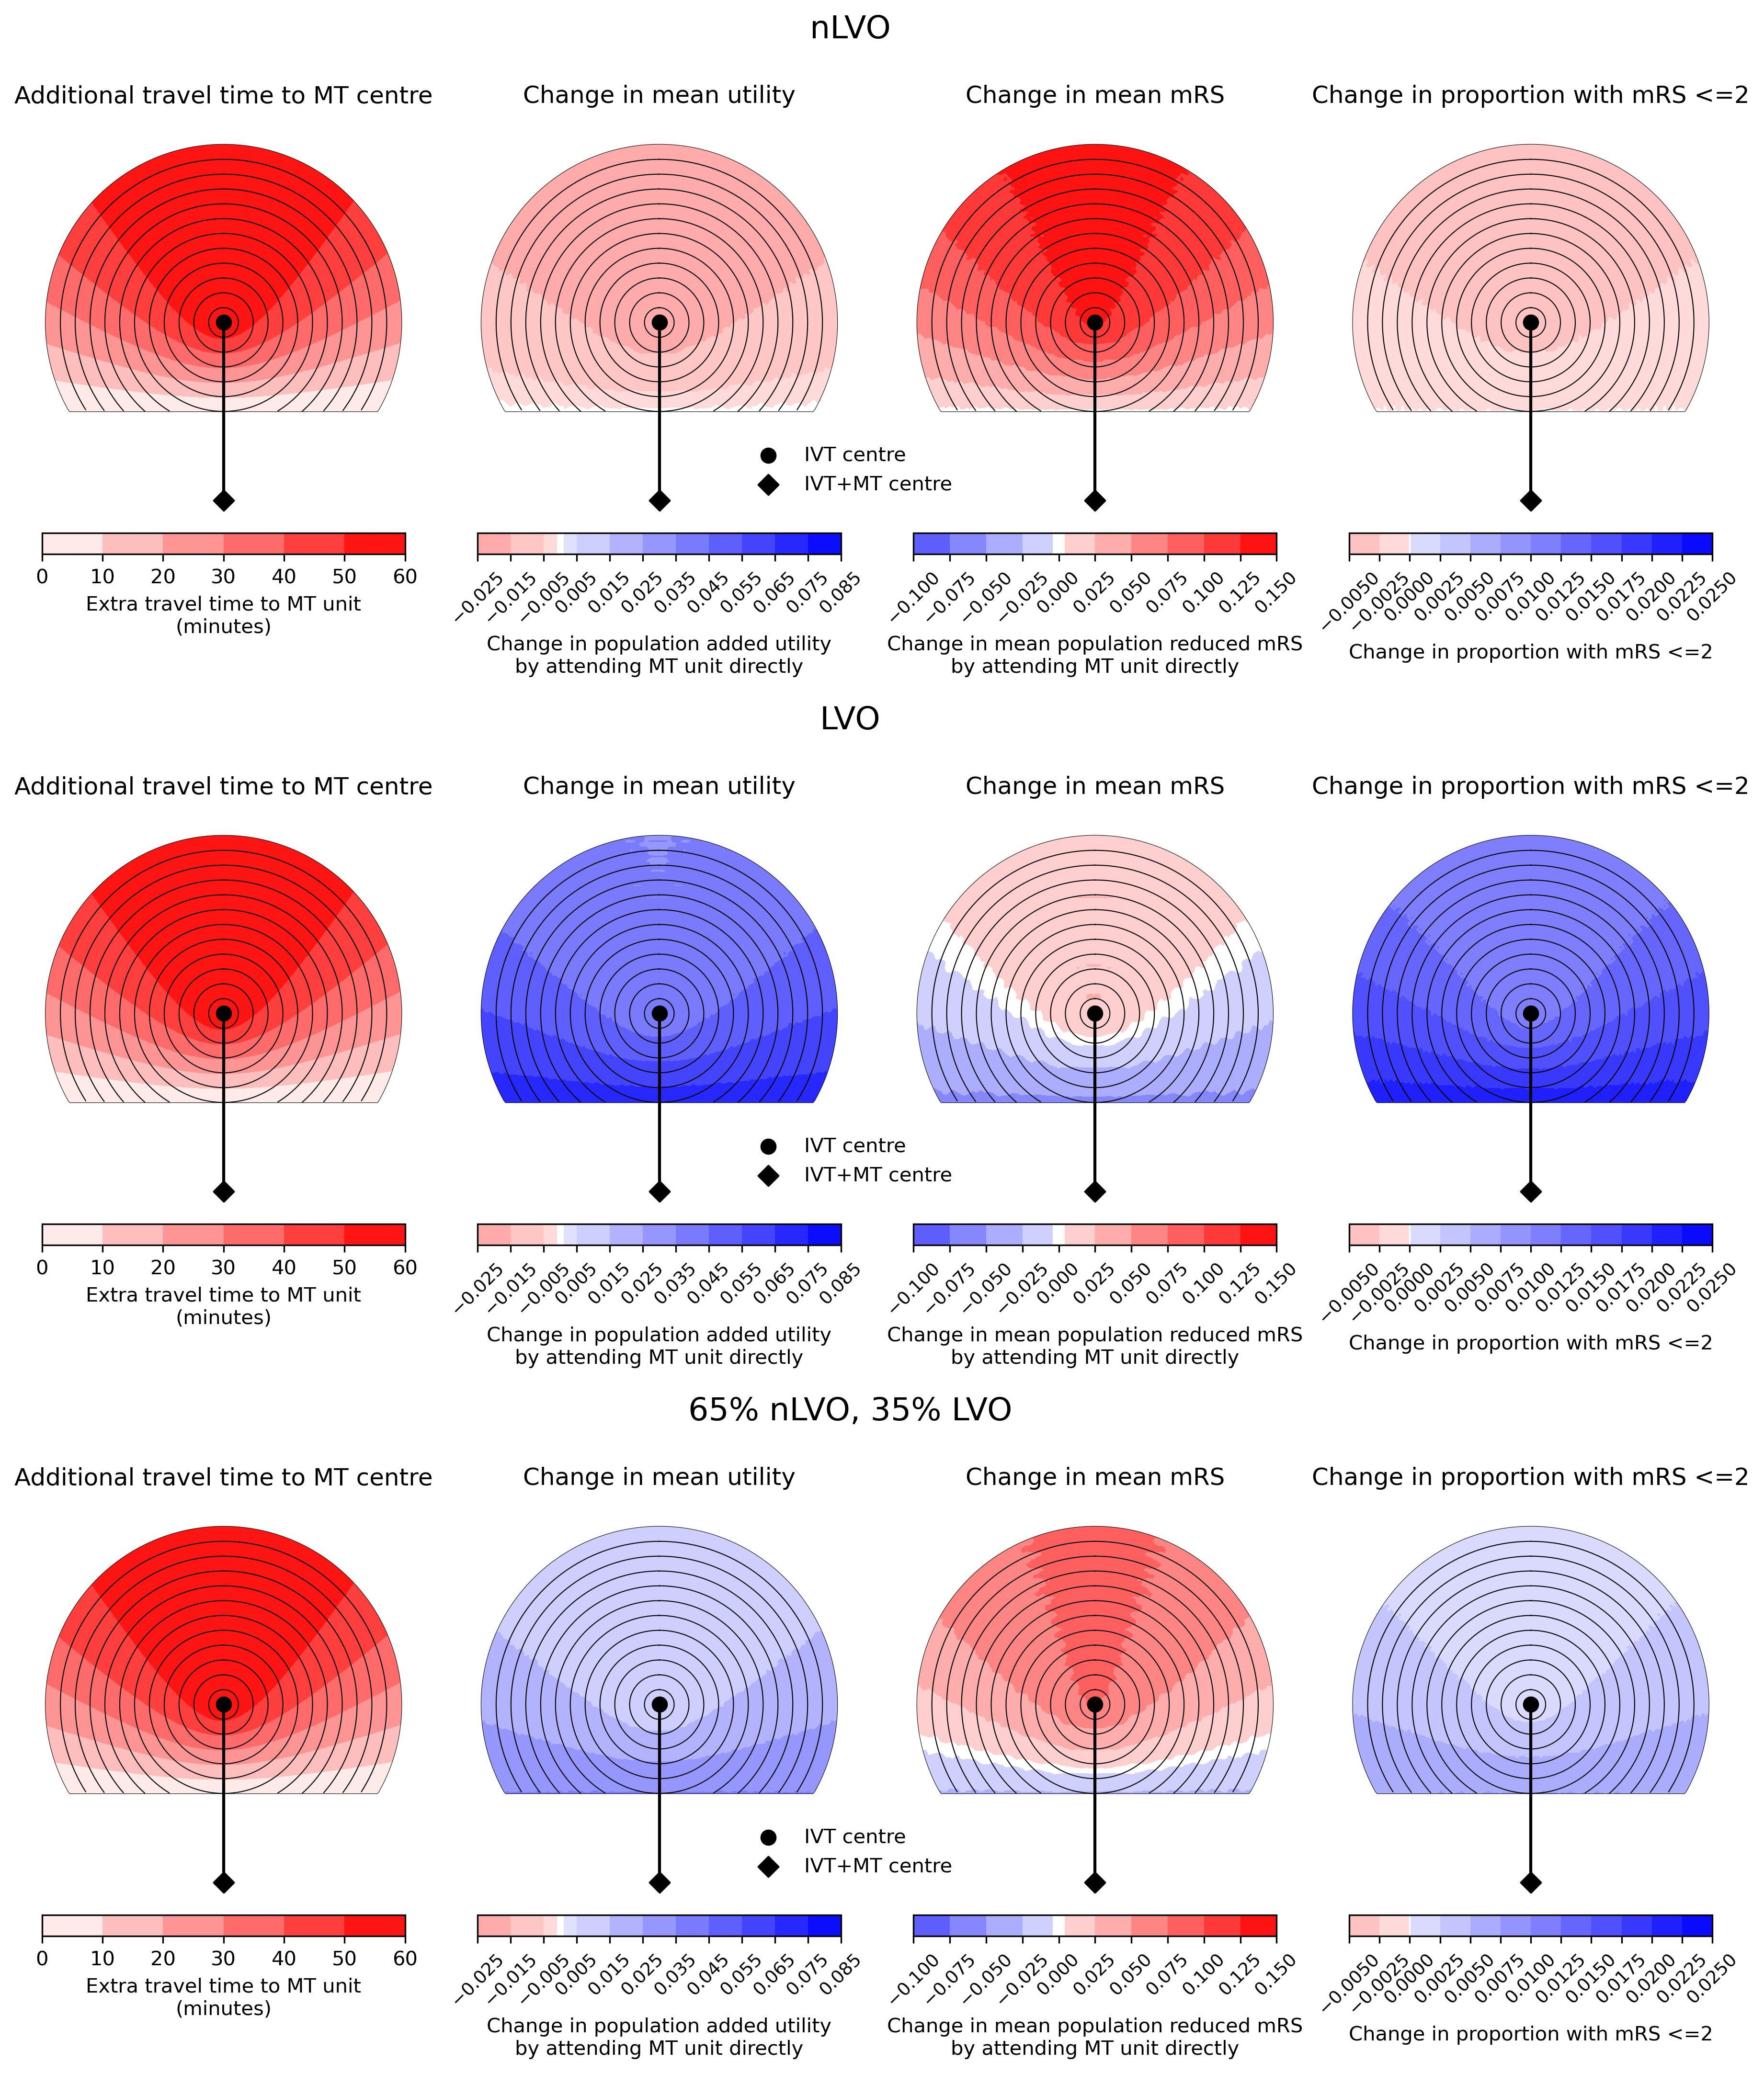
\includegraphics[width=\textwidth]{./images/circles_stroke_types}
\caption{The effect of bypassing an IVT-only unit in order to travel directly to a MT-capable unit that is 60 minutes away from the IVT-only unit. Top to bottom: results for 1) nLVO, 2) LVO, and a 3) mixed population of 65\%nLVO and 35\% LVO. Left to right: effect of bypass on 1) additional travel time to MT unit, 2) change in mean utility, 3) change in mean mRS, 4) Change in proportion with an oytcome of mRS0-2. Arrival-to-IVT is assumed to take 30 minutes, and arrival to MT is assumed to take 90 minutes. An ambulance is assumed to arrive at the patient 60 minutes after stroke onset. Drip and ship is assumed to cause a 60 min delay to MT in additional to transfer time. Concentric circles represent 5 minutes travel time intervals from IVT-only unit. Blue shades represent benefit, red shades represent disbenefit.}
\label{fig:circles}
\end{figure}

\begin{figure}
\centering
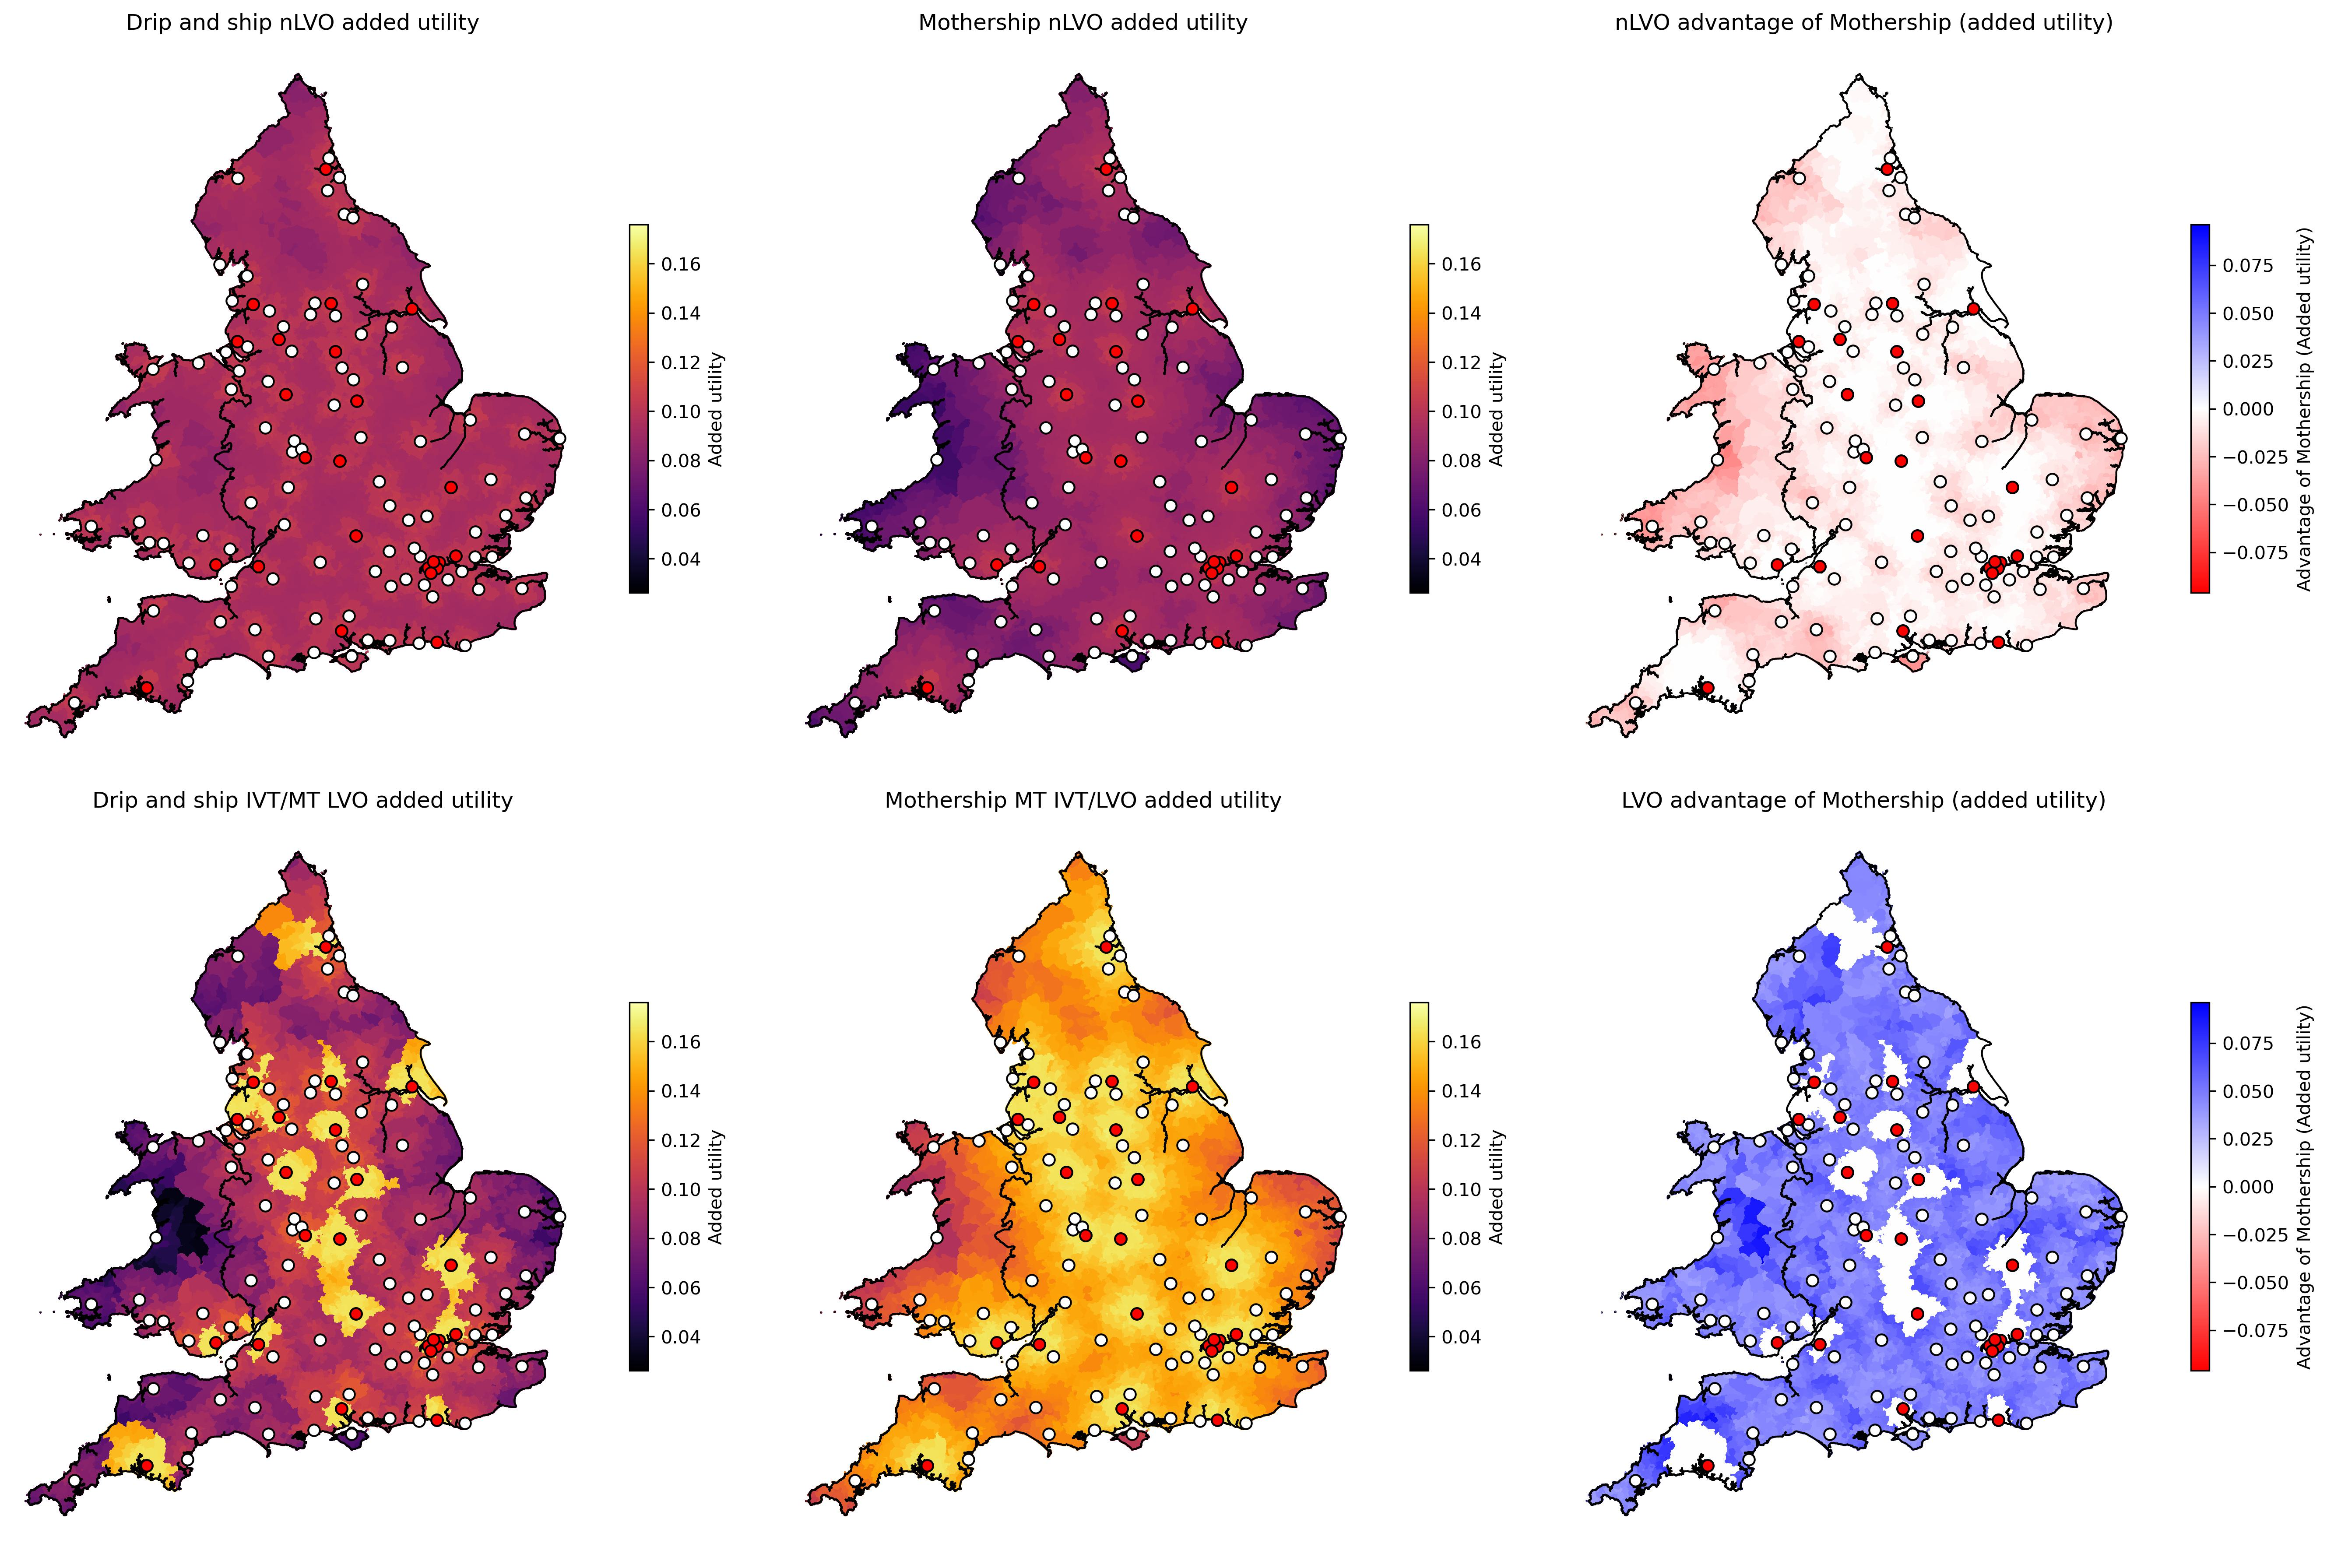
\includegraphics[width=\textwidth]{./maps/added_utility_six_in_one}
\caption{Added utility from patients treated with IVT and/or MT. Top: nLVO treated with IVT. Bottom: LVO treated with IVT and/or MT. Left: Drip and ship. Middle: Mothership. Right: advantage of mothership over drip and ship. Arrival-to-IVT is assumed to take 30 minutes, and arrival to MT is assumed to take 90 minutes. An ambulance is assumed to arrive at the patient 60 minutes after stroke onset. Drip and ship is assumed to cause a 60 min delay to MT in additional to transfer time. White circles show locations of IVT-units, and red circles show locations of IVT/MT units.}
\label{fig:added_utility_six_in_one}
\end{figure}

\begin{figure}
\centering
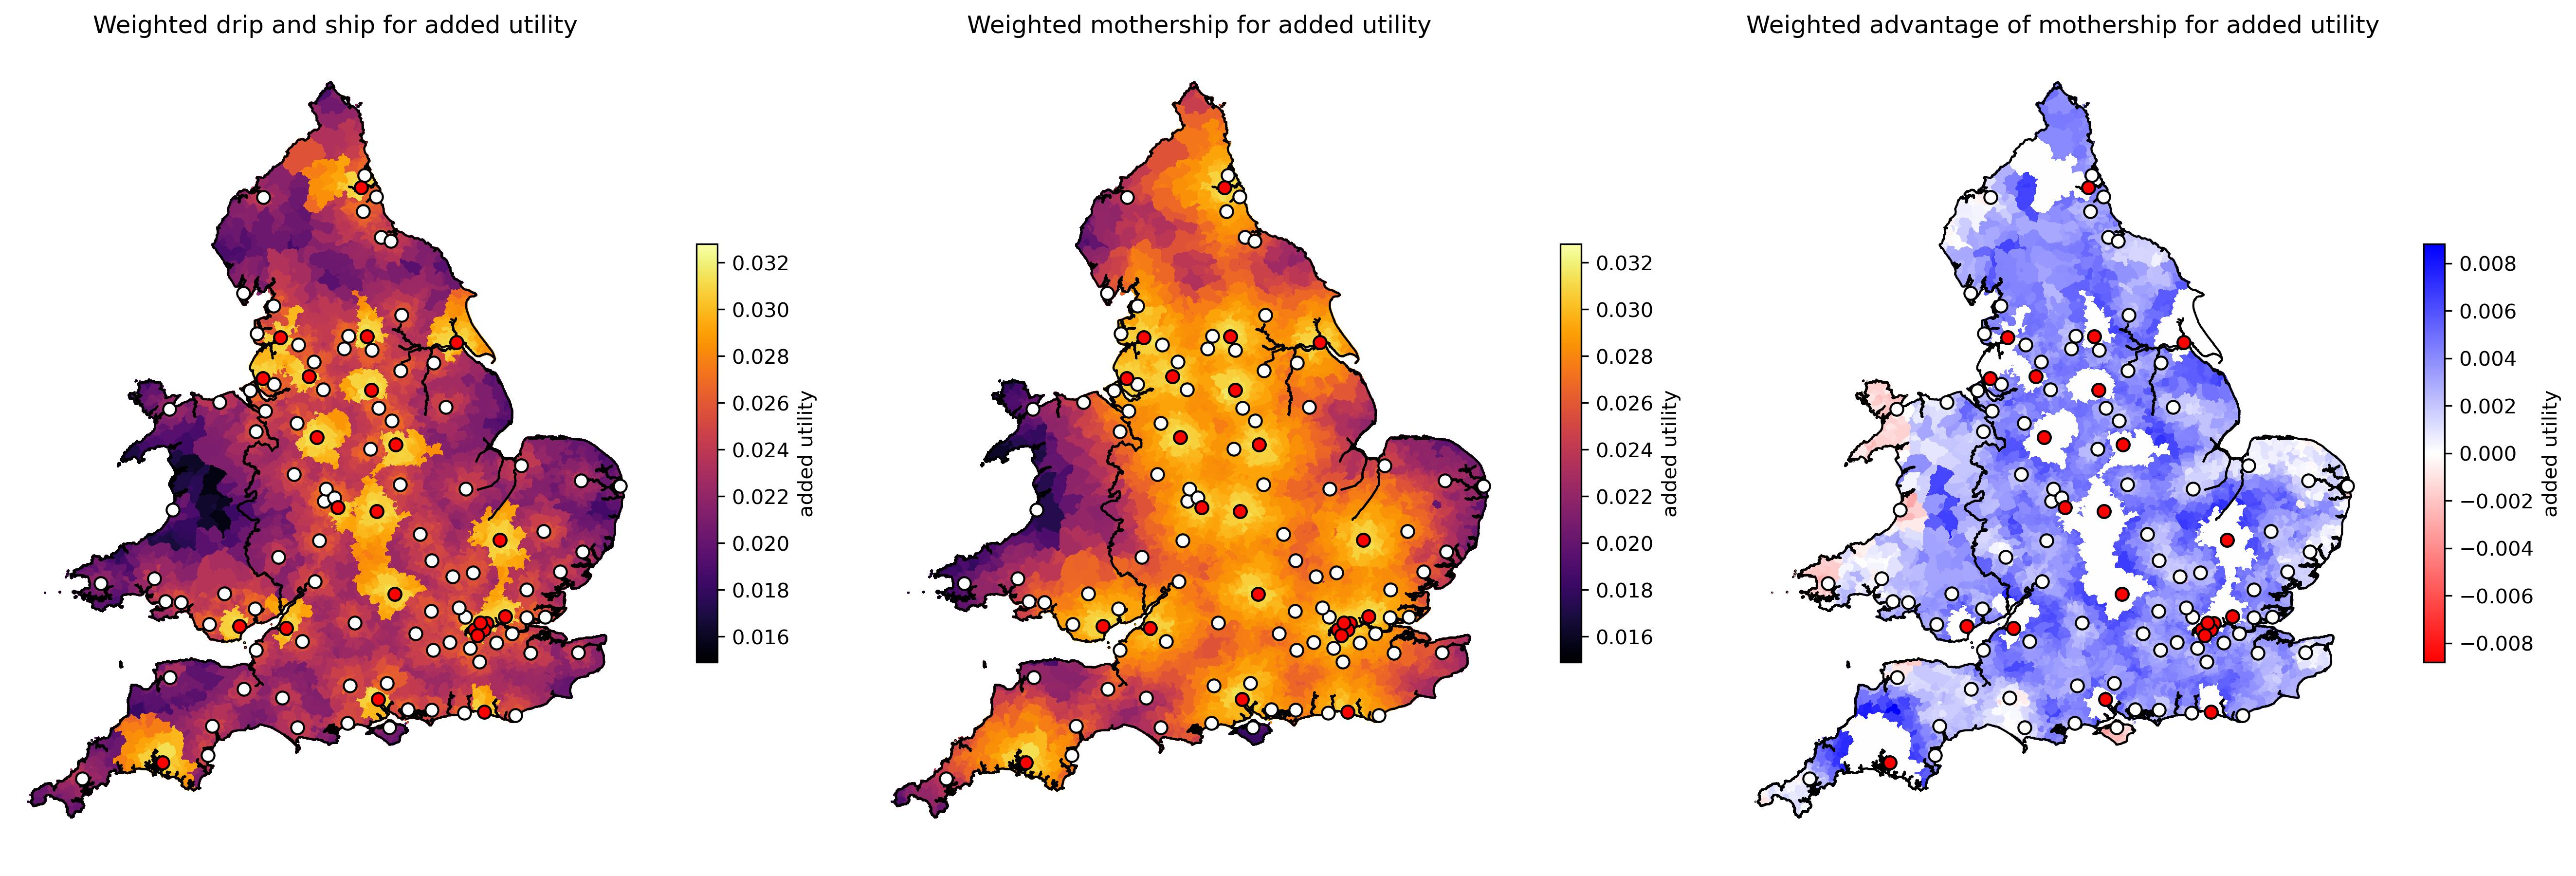
\includegraphics[width=\textwidth]{./maps/added_utility_weighted_results}
\caption{Added utility from a mixed population of nLVO (65\%) and LVO (35\%) patients treated with IVT and/or MT. Left: Drip and ship. Middle: Mothership. Right: advantage of mothership over drip and ship. Arrival-to-IVT is assumed to take 30 minutes, and arrival to MT is assumed to take 90 minutes. An ambulance is assumed to arrive at the patient 60 minutes after stroke onset. Drip and ship is assumed to cause a 60 min delay to MT in additional to transfer time. White circles show locations of IVT-units, and red circles show locations of IVT/MT units.}
\label{fig:added_utility_net}
\end{figure}
